\section{Further empirical studies}\label{app:studies}

This appendix reports the three studies summarized in Section~\ref{sec:further}. Each
applies the estimator of Section~\ref{sec:method} without modification; only the declared
grouping variable $\phi$ changes. Appendices~\ref{app:vgmain} and~\ref{app:vgvisual} stay
in relation prediction but replace the released checkpoints of
Section~\ref{sec:sggaudit} with predictors built to isolate particular kinds of
information; Appendix~\ref{app:lt} moves to long-tailed classification in two different
data modalities.

\subsection{Relation prediction with controlled predictors}\label{app:vgmain}\label{sec:data}

We work with Visual Genome \cite{krishna2017visual} in the PredCls regime
\cite{xu2017scene}, where ground-truth boxes and object labels are supplied and
the model has only to predict one of 50 predicate labels for each ordered object pair.
The predictors of this section are audited on a VG150-\emph{style} dataset we build
directly from the released relationship annotations: the 150 most frequent object
classes and 50 most frequent predicates form the vocabulary, and images are split
$70/30$ into a pool for fitting the compared predictors and a pool on which the audit
runs. We use this reconstruction rather than the canonical VG150 release because these
predictors are trained here from annotations alone; Section~\ref{sec:sggaudit} audits
\emph{released third-party checkpoints} on the canonical split itself, so both settings
appear in the paper and neither is asked to stand for the other. The reconstruction
provides 532,987 training and 229,605 test relations, drawn from 65,228 and 27,955
images respectively, and the cell throughout is
$\phi=(\text{subject class},\text{object class})$, two real examples of which appear in
Figure~\ref{fig:samples}. Of the 8,614 cells present in the test split, 6,346 contain at
least two relations and are therefore identified; the remaining 2,268 are singletons,
which WAGER excludes and reports rather than smoothing over, leaving 227,337 relations
(99.0\%) under audit.

The five predictors are deliberately constructed so that each exposes a different kind
of information. FREQ is the training-count distribution conditioned on the class pair,
with add-one smoothing and a subject-marginal and then global backoff for class pairs
unseen in training; FREQ+OVERLAP adds to it a single binary box-overlap indicator.
MLP-CLASS consumes fixed subject and object class embeddings, which makes it a function
of $\phi$ alone; MLP-SPATIAL extends those embeddings with 12 normalized box-geometry
features covering relative centre, scale, aspect, intersection, containment and IoU,
while MLP-SPATIAL+ both widens the network and trains longer (Appendix
\ref{app:implementation} lists every architecture and schedule), so its increment over
MLP-SPATIAL reflects capacity and optimization jointly rather than capacity alone. Each
is trained once on the training split, and WAGER thereafter consumes nothing but their
cached test distributions, scored quadratically with image-clustered intervals and 499
within-cell cyclic randomizations, whose smallest attainable $p$-value is
$1/500=.002$; table entries of $.002$ are at this granularity floor and should be read
as $p\le.002$. With confidence intervals as the primary uncertainty statement and every
significant effect many standard errors from zero, we do not additionally adjust the
diagnostic $p$-values for the number of reported comparisons.

\begin{figure*}[t]
\centering
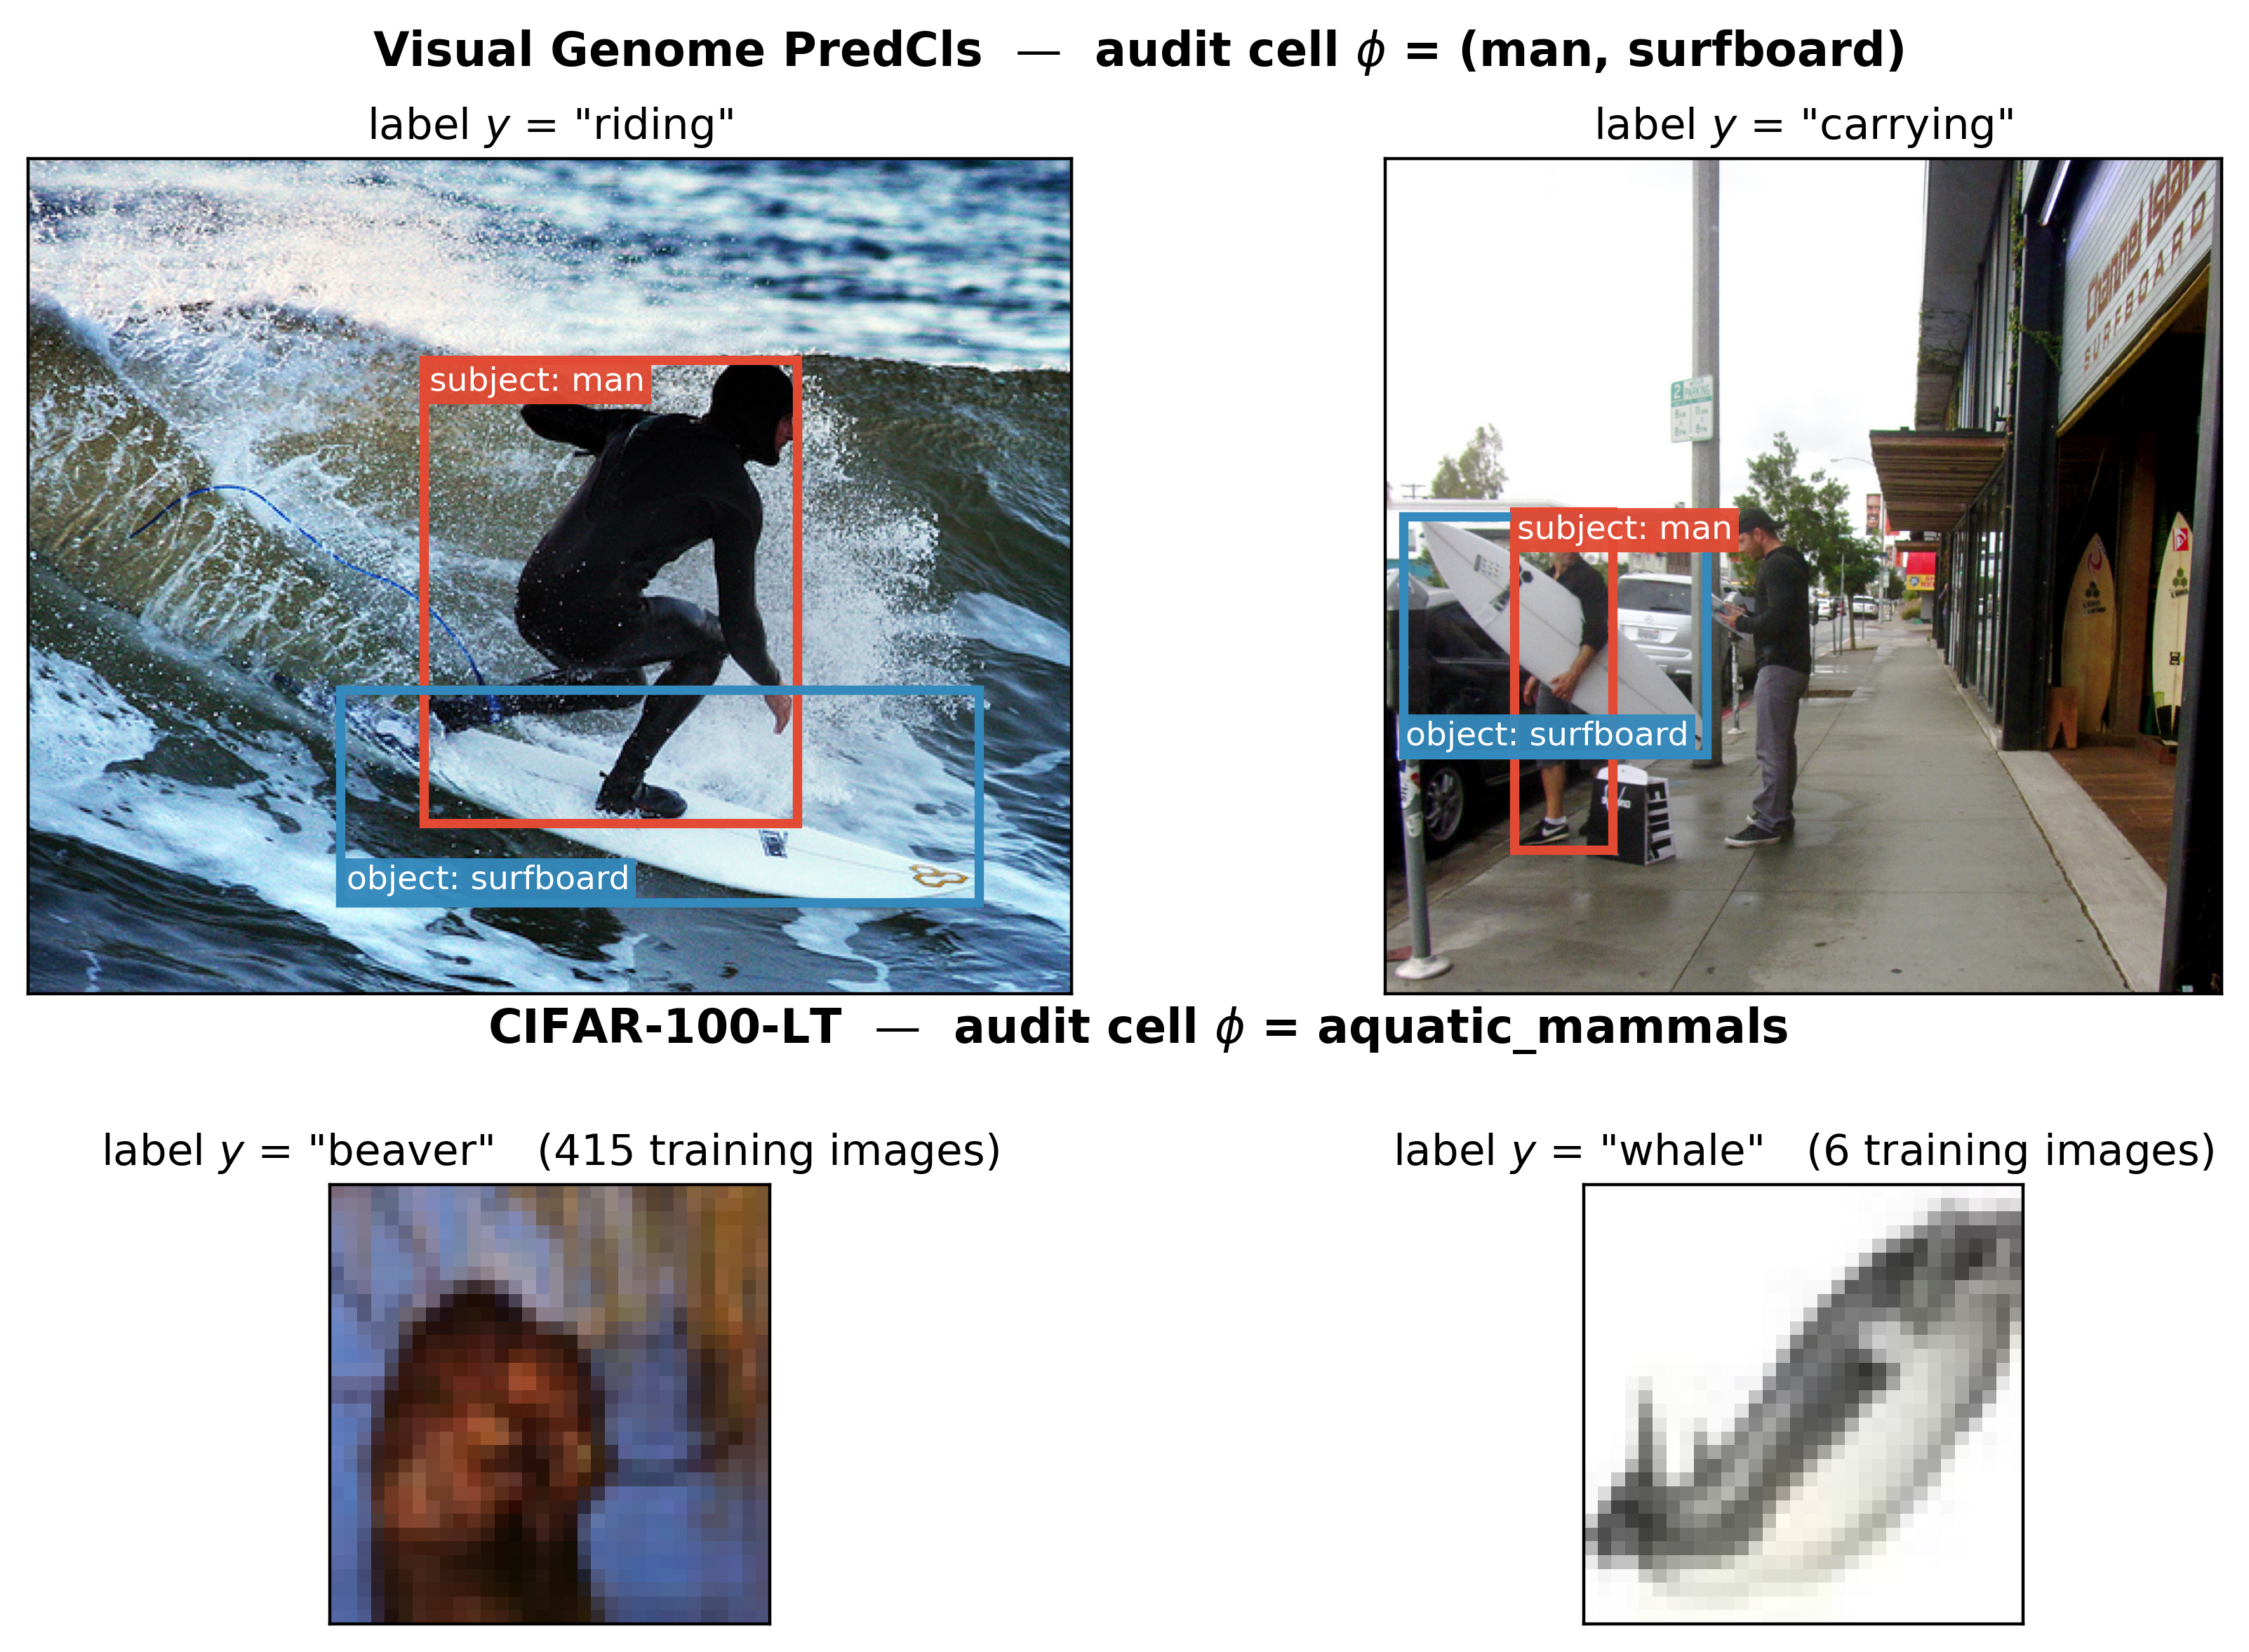
\includegraphics[width=\textwidth]{figures/fig6_dataset_samples.png}
\caption{\textbf{What an cell contains, on both benchmarks.} Each row shows two
real test examples that share the same declared grouping variable $\phi$ but carry
different labels -- precisely the configuration within-cell transport exploits.
\emph{Top:} two Visual Genome relations from the cell $\phi=(\text{man},
\text{surfboard})$. The class pair is identical and therefore cannot distinguish
``riding'' from ``carrying''; only the image content can, which is what
$\Delta R$ is designed to credit. Boxes are the annotated subject (red) and object
(blue) regions that MLP-SPATIAL turns into geometry features and MLP-VISUAL crops and
encodes with CLIP. \emph{Bottom:} two CIFAR-100 test images from the superclass
$\phi=\text{aquatic\_mammals}$, drawn from opposite ends of the long-tailed training
distribution ($415$ versus $6$ training images). Crossing the labels within a row
preserves the cell and its label histogram while destroying which prediction belongs
with which instance.}
\label{fig:samples}
\end{figure*}

\begin{table}[t]
\centering
\caption{Frozen-model top-1 accuracy on VG150 PredCls. Similar accuracies do not reveal
whether the difference is prior-fit.}
\label{tab:accuracy}
\begin{tabular}{@{}lr@{}}
\toprule
Model & Accuracy \\
\midrule
FREQ & 0.6564 \\
FREQ+OVERLAP & 0.6545 \\
MLP-CLASS & 0.6554 \\
MLP-SPATIAL & 0.6639 \\
MLP-SPATIAL+ & 0.6674 \\
\bottomrule
\end{tabular}
\end{table}

\subsection{Gain attribution for the controlled predictors}\label{sec:results}

The central result is collected in Table~\ref{tab:wager-results} and
Figure~\ref{fig:results}. MLP-CLASS improves on FREQ by $0.03386$ of quadratic score,
yet because its gain vector is constant inside every class-pair cell, the estimator
assigns that entire improvement to prior transport and precisely nothing to instance
resolution. The zero is worth dwelling on: it follows algebraically from the construction
rather than from a learned baseline happening to pass a sanity check.

Adding box geometry changes the picture. MLP-SPATIAL gains $0.04270$ over FREQ, of which
$0.02832$ survives label transport and $0.01439$ is within-group resolution (CI
$[0.01373,0.01504]$). More revealing still is the direct comparison against MLP-CLASS,
where the total gain falls to $0.00885$ only because prior fitting deteriorates by
$0.00554$ even as the resolution gain from spatial features rises by $0.01439$. The resulting resolution share
of 1.63 records a genuinely useful instance-specific change that the aggregate score
partly conceals behind a worse prior component, and it is exactly the configuration that
a ratio confined to $[0,1]$, or thresholded at $0.5$, would misdescribe.

The remaining two comparisons bracket the interesting range. MLP-SPATIAL+ adds $0.00374$
over MLP-SPATIAL, nearly all of it resolution at $0.00321$ (CI $[0.00289,0.00353]$),
whereas FREQ+OVERLAP supplies the opposite caution: its overlap indicator does create a
small positive resolution term, but the accompanying negative prior term is larger, so
the model ends up worse overall. Using image-derived information is thus never treated
as an improvement in itself; both channels are reported, signs included.

\paragraph{Reading the magnitudes.} Quadratic-score units are not ones most readers
calibrate by eye, so it is worth anchoring them in the rank-based metrics this
literature reports. Where both channels point the same way the correspondence is
straightforward: MLP-SPATIAL-S's $\widehat{\Delta R}=+0.01023$ over MLP-CLASS-S
accompanies $+0.51$ points of top-1 predicate accuracy, $+0.60$ of mean reciprocal rank
and $+0.86$ of recall@5, so in these data a hundredth of quadratic-score gain is worth
roughly half an accuracy point. The resolution channel is not, however, a re-description
of any rank metric, and the real-pixel comparison of Appendix~\ref{app:vgvisual} is
where that becomes visible: there $\widehat{\Delta R}=+0.00641$ while top-1 accuracy
falls by $3.07$ points and recall@5 by $2.21$. Prior-matching both models before scoring
narrows the accuracy gap to $2.17$ points without closing it. The rank metrics aggregate
the two channels into one number; when the channels carry opposite signs, as they do
here, no single such number can represent both, which is precisely the situation the
decomposition exists to report.

\begin{table*}[t]
\centering
\caption{WAGER decomposition on 227,337 identified VG150 PredCls relations. Gains use
the quadratic score. CI is image-cluster robust; $p$ is the 499-shift relation-level
randomization diagnostic (granularity floor $.002$). ``--'' denotes an undefined share
because total gain is negative. The MLP-CLASS row's zero-width interval is exact by
construction, not a sampling statement: a gain vector constant within every cell makes
the antisymmetric kernel identically zero (Theorem~\ref{thm:population}), so no
variability exists for the interval to measure.}
\label{tab:wager-results}
\resizebox{\textwidth}{!}{%
\begin{tabular}{@{}llrrrrr@{}}
\toprule
New model & Old model & $\widehat{\Delta T}$ & $\widehat{\Delta P}$ &
$\widehat{\Delta R}$ (95\% CI) & $\widehat\rho$ & $p$ \\
\midrule
FREQ+OVERLAP & FREQ & $-0.01229$ & $-0.01430$ & $0.00202\,[0.00168,0.00235]$ & -- & .002 \\
MLP-CLASS & FREQ & $0.03386$ & $0.03386$ & $0.00000\,[0.00000,0.00000]$ & 0.00 & .724 \\
MLP-SPATIAL & FREQ & $0.04270$ & $0.02832$ & $0.01439\,[0.01373,0.01504]$ & 0.34 & .002 \\
MLP-SPATIAL+ & FREQ & $0.04644$ & $0.02885$ & $0.01760\,[0.01686,0.01834]$ & 0.38 & .002 \\
MLP-SPATIAL & MLP-CLASS & $0.00885$ & $-0.00554$ & $0.01439\,[0.01373,0.01504]$ & 1.63 & .002 \\
MLP-SPATIAL+ & MLP-SPATIAL & $0.00374$ & $0.00053$ & $0.00321\,[0.00289,0.00353]$ & 0.86 & .002 \\
\bottomrule
\end{tabular}
}
\end{table*}

\begin{figure*}[t]
\centering
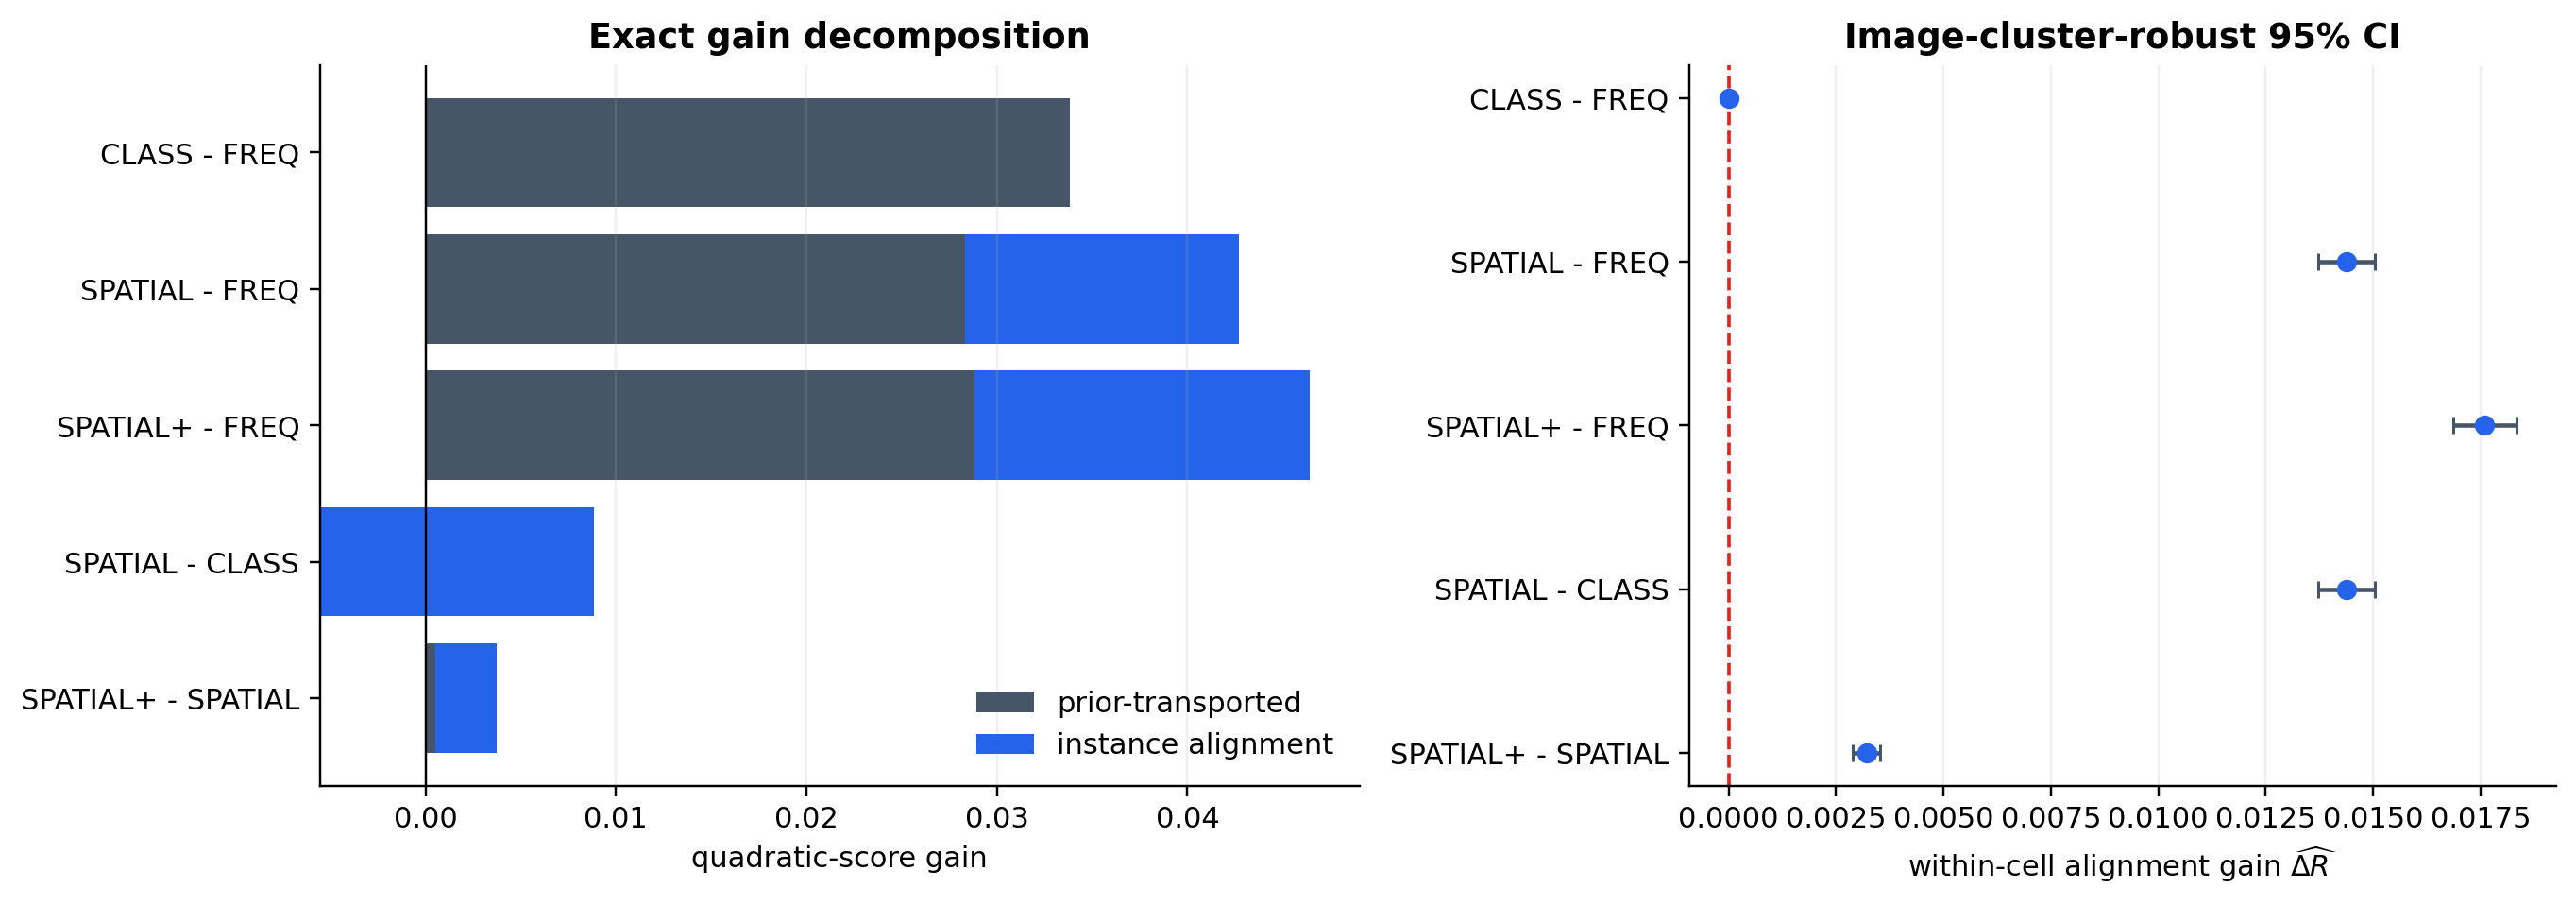
\includegraphics[width=\textwidth]{figures/fig4_new_results.png}
\caption{\textbf{Direct model-pair attribution.} Left: exact decomposition of each
positive gain into prior-fit and within-group resolution components (the negative
prior term for SPATIAL--CLASS extends left of zero). Right: primary resolution estimates
with image-cluster-robust intervals.}
\label{fig:results}
\end{figure*}

\paragraph{Reading $\widehat{\Delta T}$ as a comparative forecast test.} Corollary
\ref{cor:dm} identifies $\widehat{\Delta T}$ and its image-clustered interval in Table
\ref{tab:wager-results} as exactly a grouped Diebold--Mariano statistic and interval for
each pair's paired score differential, so every row already reports what that classical
test would report. What it does not report is the next two columns: whether MOTIFS-TDE
(Section~\ref{sec:sggaudit}) or MLP-SPATIAL beat their baseline for a reason a
frequency-only remodeling of the same benchmark could not reproduce, which is the
question $\widehat{\Delta P}$ and $\widehat{\Delta R}$ answer and DM/GW do not ask.

\subsection{Sensitivity analyses}\label{sec:ablations}

For MLP-SPATIAL versus MLP-CLASS, the conclusion survives every planned sensitivity
check (Table~\ref{tab:sensitivity}). Changing from the quadratic to a probability-floored
log score changes scale ($0.01439$ to $0.06536$) but not sign or significance.
Coarsening $\phi$ from the class pair to subject class increases the credited resolution
to $0.02181$. Proposition~\ref{prop:coarsen} identifies why: the coarser cell's estimate
equals the class-pair estimate's conditional average plus a between-class-pair covariance
term, and that term is positive here, meaning some of the credited gain reflects
class-pair-level structure that the finer audit had already correctly assigned to
$\Delta P$. This is precisely the sense in which the class-pair audit is the conservative
choice: it is not that coarsening is wrong, but that it cannot be assumed neutral, and
only the finer partition's estimate isolates resolution gain net of every prior regularity
expressible in $\phi$. The same class-pair-versus-subject-only pair also instantiates
Proposition~\ref{prop:sensitivity} directly, with the subject class playing the role of
the unrecorded confounder $Z$: Table~\ref{tab:sensitivity-numeric} in
Section~\ref{sec:sensitivity} reports that the resulting bias of $0.00742$ is comfortably
inside the Cauchy--Schwarz bound, though the bound is loose enough at $K=50$ that it
would remain satisfied for a $\bar\rho$ three orders of magnitude smaller than one.
Raising the minimum cell size from 2 to 5, 10, and 20 yields
$0.01395$, $0.01330$, and $0.01225$; all cluster-robust lower limits remain positive.
The procedure itself has no smoothing strength, split fraction, or decision threshold
to tune.

\begin{table}[t]
\centering
\caption{Sensitivity of the MLP-SPATIAL vs.\ MLP-CLASS decomposition to score, audit
granularity, and minimum cell size. CI is image-cluster robust on $\widehat{\Delta R}$.}
\label{tab:sensitivity}
\begin{tabular}{@{}llrrr@{}}
\toprule
Factor & Setting & $\widehat{\Delta T}$ & $\widehat{\Delta R}$ (95\% CI) & Cells \\
\midrule
Score & Brier (default) & $0.00885$ & $0.01439\,[0.01373,0.01504]$ & 6346 \\
Score & Log (floored) & $0.04297$ & $0.06536\,[0.06294,0.06779]$ & 6346 \\
Audit cell & class pair (default) & $0.00885$ & $0.01439\,[0.01373,0.01504]$ & 6346 \\
Audit cell & subject only & $0.00943$ & $0.02181\,[0.02079,0.02283]$ & 150 \\
Min.\ cell size & 2 (default) & $0.00885$ & $0.01439\,[0.01373,0.01504]$ & 6346 \\
Min.\ cell size & 5 & $0.00772$ & $0.01395\,[0.01329,0.01462]$ & 4060 \\
Min.\ cell size & 10 & $0.00683$ & $0.01330\,[0.01262,0.01398]$ & 2744 \\
Min.\ cell size & 20 & $0.00570$ & $0.01225\,[0.01155,0.01295]$ & 1757 \\
\bottomrule
\end{tabular}
\end{table}

\subsection{Real-pixel signal on Visual Genome}\label{app:vgvisual}\label{sec:vgvisual}

None of the models in Appendices~\ref{app:vgmain}--\ref{sec:ablations} ever sees an image.
They are functions of the declared class pair and, in the case of MLP-SPATIAL(+), of box
coordinates recorded in the annotation. Since box geometry serves only as a proxy for
what an image contains, a sceptical reader is entitled to ask whether the resolution
channel is responding to genuine pixel evidence or merely to that proxy.
Figure~\ref{fig:samples} sharpens the question: the cell
$\phi=(\text{man},\text{surfboard})$ holds both ``riding'' and ``carrying'', and although
their box configurations certainly differ, what actually distinguishes the two relations
is what the photograph shows.

MLP-VISUAL is introduced to answer it. Subject and object regions are cropped from the
original Visual Genome image and each is encoded by a frozen CLIP ViT-B/32 image encoder
\citep{radford2021learning}, after which the two $512$-dimensional embeddings are
concatenated with the class embeddings that MLP-CLASS already uses and passed to a small
trained head of 256 and 128 units. Because CLIP itself is never fine-tuned, whatever
resolution the model gains reflects information its pretraining had already recovered
from pixels and the head has merely matched to an SGG label, rather than representation
learning performed on Visual Genome.

\paragraph{Matched training data.} We report this comparison apart from
Table~\ref{tab:wager-results} rather than as an additional row, for a reason that is
itself an instance of the paper's argument. Encoding every training relation with CLIP is
expensive enough that MLP-VISUAL must be trained on a subsample, and setting a subsampled
model against the full-data MLP-SPATIAL would confound feature content with training-set
size so thoroughly that a disappointing result could not honestly be attributed to the
pixels. All three compared predictors are therefore retrained on a single fixed, seeded
subsample of $100{,}000$ of the $532{,}987$ training relations, and are written
MLP-CLASS-S, MLP-SPATIAL-S and MLP-VISUAL-S to mark the fact. Differing only in their
feature sets, any gap between them isolates the features. The audit continues to use the
complete $229{,}605$-relation test split with the same class-pair $\phi$ and
image-clustered intervals, so its numbers remain directly comparable with the main
analysis. The sampling procedure, the crop-deduplication scheme and the count of images
that could not be retrieved are given in Appendix~\ref{app:implementation}.

\paragraph{Result.} Judged by any aggregate measure, the CLIP model is the worst of the
three. Its top-1 accuracy is $0.6161$ against $0.6467$ for MLP-SPATIAL-S and $0.6416$ for
MLP-CLASS-S, and its quadratic score is lower still, falling $0.04655$ below
MLP-SPATIAL-S. An evaluator working from either number would conclude that replacing box
geometry with pixel content had simply made the predictor worse, and would discard it.

The decomposition in Table~\ref{tab:vgvisual} and Figure~\ref{fig:vgvisual} contradicts
that reading on the axis the paper cares about. Against MLP-SPATIAL-S the CLIP model
loses $0.05296$ of prior-fit gain while \emph{gaining} $0.00641$ of instance
resolution (95\% CI $[0.00514,0.00769]$, randomization $p=.002$), so its entire deficit
sits in the prior channel and its instance-level discrimination is significantly better,
not worse. The comparison against the class-only baseline tells the same story more
plainly: pixels buy $0.01665$ of resolution where box geometry buys $0.01023$, and the
two intervals are far apart. Real image content therefore carries more instance-specific
signal than the geometric proxy standing in for it, which is precisely what
Appendix~\ref{app:vgvisual} set out to test.

Why the prior channel collapses has a plausible mechanism, though we state it as a
hypothesis rather than a finding. The $1024$ CLIP dimensions dominate
the $64$ dimensions of class embedding that the head also receives, so the model fits the
class-pair frequency structure of VG150 markedly less well than a predictor built around
that structure. A benchmark whose headline metric rewards prior fitting will punish this
model, and the aggregate numbers duly do. What WAGER adds is the observation that the
punishment is not for failing to use the image; it is for failing to reproduce the
annotation prior, while using the image better than either competitor.

\paragraph{The deficit and the advantage respond to different interventions.} If the
two channels measure what they claim, they should respond asymmetrically to a post-hoc
correction that supplies prior information but no instance information. We test this by
prior matching: within each class-pair cell, a model's predictions are reweighted so
that their cell mean matches the training-count histogram, a label-shift-style
correction that uses no test labels. The correction registers, as it must, almost
entirely in the prior channel ($\Delta P=+0.02401$ against $\Delta R=+0.00111$ for the
CLIP model relative to its uncorrected self), and it cuts the CLIP model's aggregate
deficit roughly in half ($-0.04655$ to $-0.02143$) while leaving the resolution advantage
intact ($+0.00752$, or $+0.00663$ with both models corrected). A calibration-matched
audit -- temperatures fitted on a held-out image split, $T^*=1.18$ against $1.00$, so
these heads are nearly calibrated to begin with -- likewise leaves the advantage
significant at $+0.00467$ $[+0.00314,+0.00621]$. The resolution channel is therefore
neither manufacturable by prior correction nor an artifact of confidence scaling.
Conversely, the part of the deficit that prior matching removes is exactly the part a
deployment could restore by re-weighting; the remainder reflects differences in
within-cell prediction dispersion rather than in the fitted cell histogram.

This is the paper's argument running in the opposite direction from
Appendix~\ref{app:lt}. There a near-zero total gain concealed a large resolution
\emph{loss}; here a clearly negative total gain conceals a real resolution \emph{gain}. In
both cases the aggregate score is not merely imprecise but actively misleading about the
thing a vision benchmark is meant to measure, and in both cases the two channels recover
what it hides.

\begin{table}[t]
\centering
\caption{Matched-subsample real-pixel study on the full VG150 test split (coverage
$99.0\%$, as in Table~\ref{tab:wager-results}). All three predictors are trained on the
same $100{,}000$ relations and differ only in features. CI is image-cluster robust on
$\widehat{\Delta R}$; $p$ is the 499-shift randomization diagnostic.}
\label{tab:vgvisual}
\resizebox{\textwidth}{!}{%
\begin{tabular}{@{}llrrrr@{}}
\toprule
New model & Old model & $\widehat{\Delta T}$ & $\widehat{\Delta P}$ &
$\widehat{\Delta R}$ (95\% CI) & $p$ \\
\midrule
MLP-SPATIAL-S & MLP-CLASS-S   & $0.00503$  & $-0.00520$ & $0.01023\,[0.00967,0.01079]$ & .002 \\
MLP-VISUAL-S  & MLP-CLASS-S   & $-0.04152$ & $-0.05816$ & $0.01665\,[0.01534,0.01796]$ & .002 \\
MLP-VISUAL-S  & MLP-SPATIAL-S & $-0.04655$ & $-0.05296$ & $0.00641\,[0.00514,0.00769]$ & .002 \\
\bottomrule
\end{tabular}
}
\end{table}

\begin{figure*}[t]
\centering
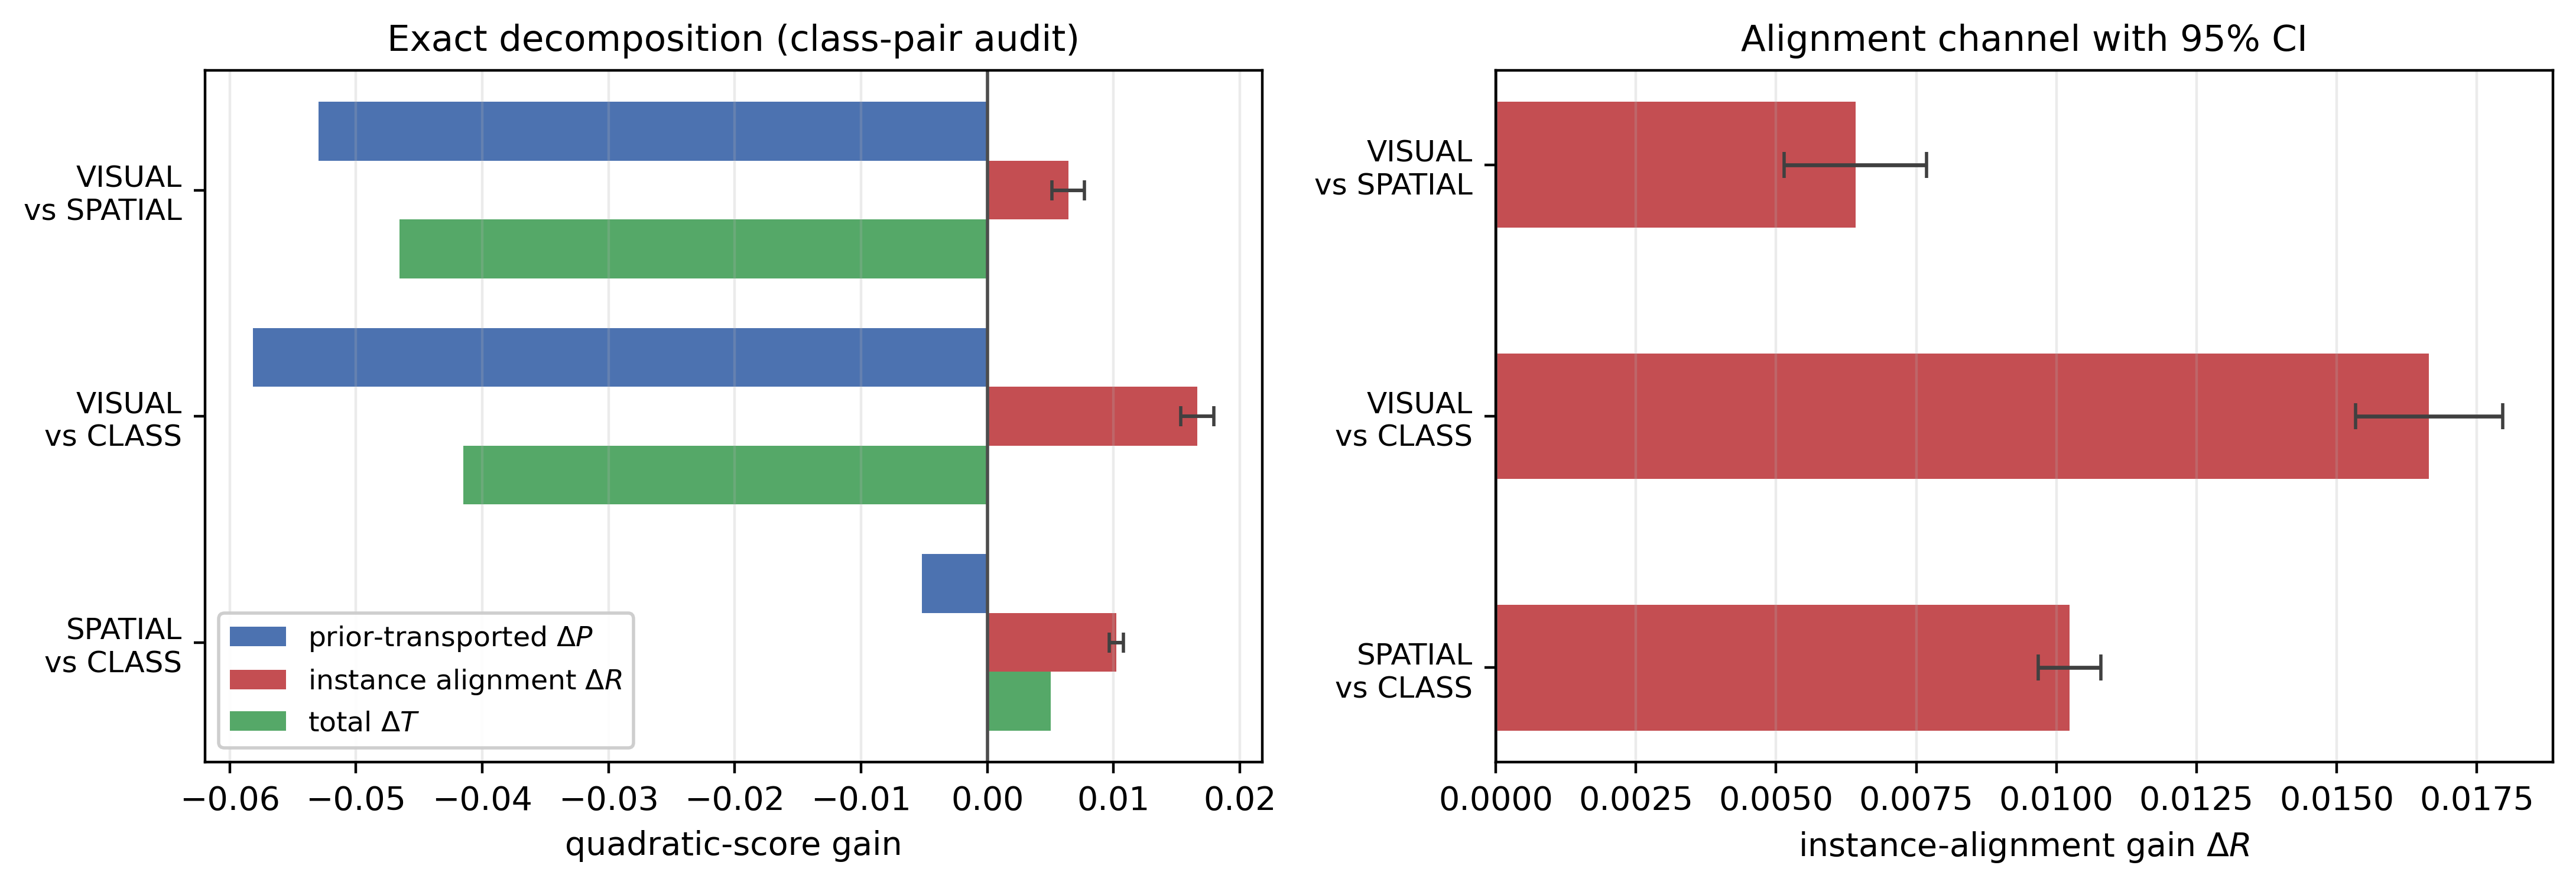
\includegraphics[width=\textwidth]{figures/fig7_vg_visual.png}
\caption{\textbf{Pixels beat geometry on resolution while losing on the aggregate.}
Left: the exact decomposition for the three matched-subsample pairs. Both comparisons
involving the CLIP model have strongly negative totals (green) driven entirely by the
prior channel (blue), while their resolution channel (red) is positive in every case.
Right: the resolution channel alone, with 95\% image-clustered intervals. Replacing box
geometry with real image content raises within-group resolution from $0.01023$ to $0.01665$
over the same class-only baseline.}
\label{fig:vgvisual}
\end{figure*}

\subsection{Long-tailed image classification}\label{app:lt}\label{sec:cifarlt}

Appendices~\ref{app:vgmain}--\ref{app:vgvisual} are all instances of one task (predicate
classification on an ordered object pair). Section~\ref{sec:related-applied} argued
that long-tailed image classification poses a structurally identical question: a
class-frequency prior can be fit better without any per-instance improvement. We test
this directly on CIFAR-100-LT \citep{cui2019classbalanced}, an exponential-imbalance
(ratio $100$) subsample of CIFAR-100's training split with the original, balanced test
split retained for evaluation. We train ResNet-32 \citep{he2016deep} classifiers that
differ only in their per-class loss weighting: a vanilla cross-entropy baseline (CE);
class-balanced effective-number re-weighting applied from initialization (CB)
\citep{cui2019classbalanced}; and the same re-weighting deferred to the final twenty
epochs (DRW) \citep{cao2019learning}. Optimizer, schedule, augmentation, epoch budget,
and seed are identical across runs (Appendix~\ref{app:implementation}).

\paragraph{Choosing $\phi$.} A declared grouping variable has to predict the label without
determining it, and this second benchmark makes the constraint unusually easy to
violate. Were $\phi$ taken to be the fine class label itself, every cell would be
label-homogeneous, within-cell transport would have nothing to cross, and
$\widehat{\Delta R}$ would come out identically zero -- an algebraic artifact wearing the
appearance of a finding. CIFAR-100's own 20 coarse superclasses avoid this, each
gathering five fine labels into a cell of $500$ balanced test images, which is
structurally the situation of a VG class-pair cell holding several predicates
(Figure~\ref{fig:samples}). Alongside the superclass audit we report two further
declared priors: the trivial coarsening to a single global cell, which audits against
the global class marginal and so instantiates Proposition~\ref{prop:coarsen} in a second
domain, and a partition into head, medium and tail training-frequency tiers. CIFAR-100
test images are independent, unlike the several relations VG draws from one photograph,
so no cluster grouping is required and the plain H\'ajek interval of
Section~\ref{sec:inference} applies directly. One semantic point matters in this domain:
transport uses each cell's \emph{test} label histogram, which on CIFAR-100-LT is
balanced. A positive $\Delta P$ here therefore records movement \emph{toward} the
balanced test marginal -- undoing the training-frequency skew -- which is precisely the
adjustment long-tailed evaluation is designed to reward; a prior-fit gain is a
description of where score was earned, not an accusation
(Section~\ref{sec:discussion}).

\paragraph{Result.} The three classifiers reach top-1 accuracies of $0.3662$ (CE),
$0.2627$ (CB) and $0.3874$ (DRW), so re-weighting from initialization degrades the
classifier substantially while the deferred schedule delivers the improvement it was
designed to produce. Table~\ref{tab:cifar} decomposes both gains against the superclass
audit.

Of the two, the class-balanced run is the more instructive, precisely because its
aggregate score conceals almost everything of interest. On the quadratic score it gains
$+0.00143$ over the baseline, a difference small enough that a reader working from the
headline number alone would reasonably conclude that re-weighting had changed very
little. The decomposition tells another story: within superclasses the
prior-fit channel improves by $+0.19713$ while within-group resolution deteriorates
by $-0.19569$ (95\% CI $[-0.20728,-0.18411]$), so the near-zero total is not a small
effect but two large ones that happen to cancel.

\paragraph{A calibration-matched regime.} A channel split of that shape could, however,
be produced by confidence scaling alone. Under the quadratic score the resolution channel
is a covariance between probability movements and labels
(Eq.~\eqref{eq:cov-id}), and a monotone recalibration moves it: softening an
overconfident model transfers score mass from the resolution to the prior channel while
adding no information about any individual image. The baseline invites exactly this
concern, assigning a mean maximum probability of $0.764$ while being correct on only
$0.3662$ of the test set. We therefore repeat the audit in a calibration-matched regime:
each model's temperature is chosen by held-out likelihood on a calibration half of the
test split ($T^*=2.85$ for CE, $3.51$ for CB, $2.61$ for DRW), the decomposition is
computed on the disjoint audit half, and the whole procedure is repeated over twenty
random splits (Table~\ref{tab:cifar-cal}). The regime's necessity is quantified by its
control row: recalibrating the baseline alone -- a transformation carrying no instance
information -- moves the channels by $+0.380$ (prior) and $-0.175$ (resolution), so the
raw split does mix calibration with discrimination.

The calibration-matched rows then separate the two schedules cleanly, and more sharply
than the raw ones. CB's resolution deficit does not shrink but widens, to
$-0.23991\,(0.00491)$: the model re-weighted from initialization has genuinely lost
within-superclass discrimination -- a real degradation that the ten-point accuracy drop
records independently -- and its near-zero raw total reflects that loss offset by its
softer, better-calibrated confidence. DRW inverts the reading its raw split suggests.
Raw, its $+0.06712$ gain divides roughly two-thirds prior to one-third resolution;
calibration-matched, the improvement is $+0.02173\,(0.00275)$ of which
$+0.01957\,(0.00329)$ is within-group resolution while the prior channel is close to zero
($+0.00216\,(0.00410)$). What survives calibration matching is precisely the component
the deferred schedule was designed to buy -- per-instance discrimination, concentrated
on rare classes (Table~\ref{tab:cifar-tier}) -- while the apparently prior-fit
share of its raw gain was largely the calibration difference between the two runs.
Neither an accuracy difference nor an aggregate score exposes either composition, which
is the practical argument for reporting the two channels, in both regimes, instead of
their sum.

\begin{table}[t]
\centering
\caption{Raw and calibration-matched decompositions on CIFAR-100-LT at the superclass
audit. Temperatures are fitted by likelihood on a held-out calibration half of the test
split; every decomposition uses the disjoint audit half; entries are means (sd) over
twenty random splits. The final row is the control: recalibrating the baseline alone
carries no instance information yet moves both channels substantially.}
\label{tab:cifar-cal}
\resizebox{\textwidth}{!}{%
\begin{tabular}{@{}llrrr@{}}
\toprule
Comparison & Regime & $\widehat{\Delta T}$ & $\widehat{\Delta P}$ &
$\widehat{\Delta R}$ \\
\midrule
CB vs CE  & raw                 & $+0.00208\,(0.00642)$ & $+0.19635\,(0.00369)$ & $-0.19427\,(0.00632)$ \\
CB vs CE  & calibration-matched & $-0.12912\,(0.00373)$ & $+0.11079\,(0.00372)$ & $-0.23991\,(0.00491)$ \\
DRW vs CE & raw                 & $+0.06712\,(0.00865)$ & $+0.04258\,(0.00463)$ & $+0.02454\,(0.00685)$ \\
DRW vs CE & calibration-matched & $+0.02173\,(0.00275)$ & $+0.00216\,(0.00410)$ & $+0.01957\,(0.00329)$ \\
\midrule
CE recalibrated vs CE & control & $+0.20495\,(0.00420)$ & $+0.37960\,(0.00268)$ & $-0.17464\,(0.00455)$ \\
\bottomrule
\end{tabular}
}
\end{table}

\paragraph{Seeds, imbalance ratios, and a post-hoc arm.} A decomposition computed from
one trained pair carries only test-set sampling uncertainty, which is not the uncertainty
relevant to a claim about a training \emph{method}. We therefore retrained the triple at
two further seeds at the primary ratio and at imbalance ratios $10$ and $50$, and added a
fourth arm: post-hoc logit adjustment (LA), which divides the baseline's predictions by
the training class prior without retraining \citep{menon2021long}. Every configuration is
audited in both regimes; Table~\ref{tab:cifar-robust} reports the calibration-matched
resolution channel, which is the one the preceding paragraphs interpret.

Three things follow. First, the class-balanced run's resolution loss is not a
misconfiguration but a systematic function of imbalance severity: $-0.069$ at ratio $10$,
$-0.244$ at $50$, and $-0.251\,(0.011)$ across three seeds at $100$, tracking an accuracy
penalty that grows from $2.3$ to $10.4$ points over the same range. Second, the deferred
schedule's resolution gain is positive at every ratio and in every seed, but its magnitude
varies roughly fourfold across seeds at ratio $100$ ($+0.007$ to $+0.031$). We therefore
report the spread rather than a seed-level interval: the direction replicates, the
magnitude is seed-sensitive, and the gap between the tight within-run intervals of
Table~\ref{tab:cifar} and this across-seed spread is exactly why a method-level claim
needs replication rather than a single audit.

Third, LA is an instructive falsification of a natural expectation. A purely post-hoc
prior correction might be expected to register as almost pure prior channel, as the
within-cell prior matching of Appendix~\ref{app:vgvisual} does. It does not:
calibration-matched, LA reads as almost entirely resolution ($+0.022$ to $+0.038$) with a
prior channel near zero, while achieving the best balanced accuracy of any arm at every
ratio. The reason is visible in the construction. Dividing by the \emph{global} class
prior is not a within-superclass histogram move, because fine classes inside a superclass
differ in training frequency, and the correction it applies is multiplicative in each
example's own predicted probabilities --- it changes rankings where the model already
carried latent evidence. The two post-hoc corrections in this paper therefore land in
opposite channels, and correctly so: transport separates adjustments that act on the
cell's label histogram from adjustments that act on individual predictions.

\begin{table}[t]
\centering
\caption{Calibration-matched resolution gain across seeds and imbalance ratios, with
balanced test accuracy for each arm. LA is post-hoc logit adjustment applied to the
baseline. The class-balanced deficit scales with imbalance severity; the deferred
schedule's gain is positive throughout but seed-sensitive in magnitude; the post-hoc
correction lands in the resolution channel rather than the prior channel.}
\label{tab:cifar-robust}
\resizebox{\textwidth}{!}{%
\begin{tabular}{@{}llrrrrrrr@{}}
\toprule
& & \multicolumn{4}{c}{Top-1 accuracy} & \multicolumn{3}{c}{$\widehat{\Delta R}$ vs.\ CE (calibration-matched)} \\
\cmidrule(lr){3-6}\cmidrule(l){7-9}
Ratio & Seed & CE & CB & DRW & LA & CB & DRW & LA \\
\midrule
$10$  & 0 & $0.5388$ & $0.5154$ & $0.5447$ & $0.5497$ & $-0.06903$ & $+0.00617$ & $+0.02222$ \\
$50$  & 0 & $0.4256$ & $0.3242$ & $0.4399$ & $0.4550$ & $-0.24409$ & $+0.01903$ & $+0.03768$ \\
$100$ & 0 & $0.3662$ & $0.2627$ & $0.3874$ & $0.3959$ & $-0.23936$ & $+0.01987$ & $+0.03449$ \\
$100$ & 1 & $0.3614$ & $0.2287$ & $0.3762$ & $0.3877$ & $-0.26176$ & $+0.00748$ & $+0.02672$ \\
$100$ & 2 & $0.3687$ & $0.2481$ & $0.3968$ & $0.4024$ & $-0.25213$ & $+0.03124$ & $+0.03601$ \\
\midrule
\multicolumn{2}{@{}l}{$100$, mean (sd)} & & & & &
$-0.25108\,(0.01124)$ & $+0.01953\,(0.01188)$ & $+0.03241\,(0.00498)$ \\
\bottomrule
\end{tabular}
}
\end{table}

Where the resolution gain sits is visible in Table~\ref{tab:cifar-tier} and
Figure~\ref{fig:cifar} (raw regime, primary seed). For DRW it falls where the long-tail literature intends it to,
reaching $+0.09009$ on few-shot classes and $+0.06760$ on medium-shot ones, while
many-shot classes lose $-0.07624$ as the schedule shifts capacity away from the head.
The class-balanced run reproduces that same ordering with every level displaced
downward, its many-shot resolution collapsing to $-0.41977$. What the decomposition
supplies, then, is not only how much of a long-tail gain is real but where in the
frequency spectrum it was earned.

These numbers also provide an implementation check on real inputs. Computing the
resolution term directly from the covariance identity of Eq.~\eqref{eq:cov-id}, through a
code path that shares nothing with the transport estimator, gives $-0.19530$; multiplying
by the factor $n_c/(n_c-1)$ that Proposition~\ref{prop:attenuate} predicts, at the
$n_c=500$ of a balanced superclass cell, returns $-0.195693$ against the estimator's
$-0.19569$. The identities of Theorem~\ref{thm:population} and
Proposition~\ref{prop:attenuate} are algebraic, so this verifies the implementation
rather than the theory; the point of the check is that two independent code paths agree
to the fifth decimal on real trained models, not only on the synthetic populations used
in the unit tests.

\begin{table}[t]
\centering
\caption{WAGER decomposition on the 10,000-image balanced CIFAR-100-LT test split.
Gains use the quadratic score; CI is the H\'ajek interval on $\widehat{\Delta R}$;
$p$ is the 499-shift randomization diagnostic, one-sided for positive resolution, so the
value of $1.000$ on the CB rows records an resolution gain at the extreme negative end of
its randomization distribution.}
\label{tab:cifar}
\resizebox{\textwidth}{!}{%
\begin{tabular}{@{}llrrrr@{}}
\toprule
Comparison & Audit cell $\phi$ & $\widehat{\Delta T}$ & $\widehat{\Delta P}$ &
$\widehat{\Delta R}$ (95\% CI) & $p$ \\
\midrule
CB vs CE  & superclass (20) & $0.00143$ & $0.19713$ & $-0.19569\,[-0.20728,-0.18411]$ & $1.000$ \\
CB vs CE  & global (1)      & $0.00143$ & $0.25573$ & $-0.25430\,[-0.26801,-0.24058]$ & $1.000$ \\
CB vs CE  & tier (3)        & $0.00143$ & $0.25247$ & $-0.25103\,[-0.26453,-0.23754]$ & $1.000$ \\
\midrule
DRW vs CE & superclass (20) & $0.06606$ & $0.04206$ & $0.02400\,[0.01340,0.03460]$ & $.002$ \\
DRW vs CE & global (1)      & $0.06606$ & $0.03522$ & $0.03085\,[0.01860,0.04309]$ & $.002$ \\
DRW vs CE & tier (3)        & $0.06606$ & $0.03702$ & $0.02904\,[0.01702,0.04107]$ & $.002$ \\
\bottomrule
\end{tabular}
}
\end{table}

\begin{table}[t]
\centering
\caption{Resolution gain by training-frequency tier at the primary superclass audit.
The deferred schedule concentrates its genuine per-instance improvement on rare
classes; both methods lose resolution on the head.}
\label{tab:cifar-tier}
\begin{tabular}{@{}lrrrr@{}}
\toprule
& & \multicolumn{1}{c}{CB vs CE} & \multicolumn{2}{c}{DRW vs CE} \\
\cmidrule(l){3-3}\cmidrule(l){4-5}
Tier & $n$ & $\widehat{\Delta R}$ & $\widehat{\Delta T}$ & $\widehat{\Delta R}$ \\
\midrule
Few-shot ($<20$)        & 3000 & $-0.03337$ & $0.13785$ & $0.09009$ \\
Medium-shot ($20$--$100$) & 3500 & $-0.11075$ & $0.10799$ & $0.06760$ \\
Many-shot ($>100$)      & 3500 & $-0.41977$ & $-0.03740$ & $-0.07624$ \\
\bottomrule
\end{tabular}
\end{table}

\begin{figure*}[t]
\centering
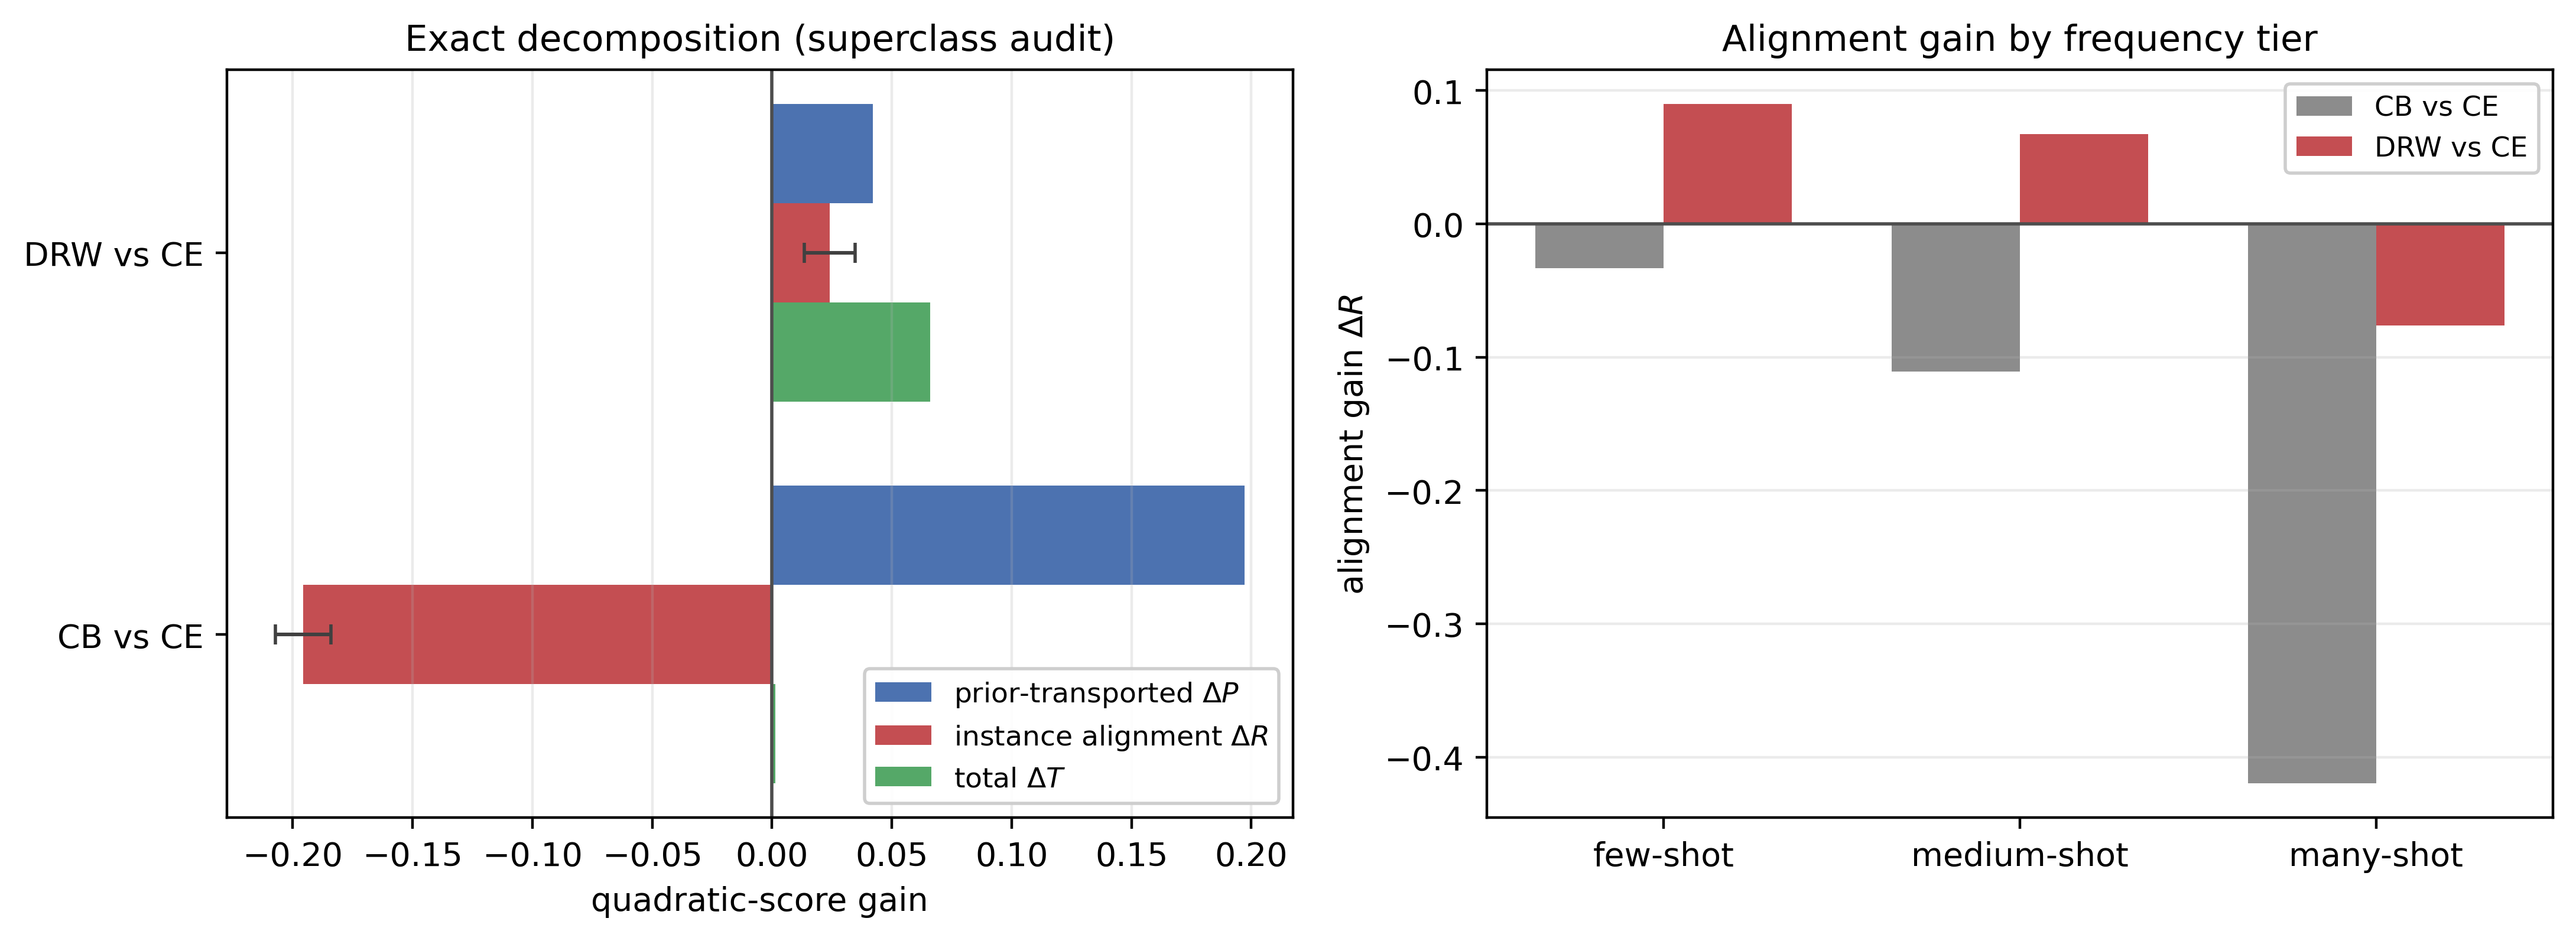
\includegraphics[width=\textwidth]{figures/fig5_cifar_lt.png}
\caption{\textbf{The same attribution transfers to a second task.} Left: exact
decomposition at the superclass audit. The CB total gain (green) is visually almost
absent at $+0.00143$ while its two channels reach $\pm0.2$ -- a near-zero aggregate
score concealing two large opposing effects. DRW's smaller total is genuinely split
between both channels. Error bars are 95\% H\'ajek intervals on $\widehat{\Delta R}$.
Right: the resolution channel by training-frequency tier, showing that DRW's genuine
per-instance gain is concentrated on rare classes and negative on the head.}
\label{fig:cifar}
\end{figure*}

Coarsening behaves as Proposition~\ref{prop:coarsen} predicts. Moving from the 20
superclass cells to a single global cell changes the credited resolution from $-0.19569$
to $-0.25430$; the difference is the between-cell covariance term, which is negative
here, so the coarse audit overstates the resolution loss by attributing to it structure
that the superclass partition correctly assigns to $\Delta P$. The finer partition is
again the conservative reading, for the same reason as in Appendix~\ref{sec:ablations}
and now in a second domain.

\subsection{Long-tailed text classification}\label{sec:textlt}

Appendices~\ref{sec:results}--\ref{app:lt} test two vision tasks that share cached
probability vectors and grouping variables grounded in class frequency or object geometry.
To test the breadth Section~\ref{sec:broader} claims -- any benchmark supplying two
models' full probability vectors, labels, and a declared discrete grouping variable -- we
apply the identical estimator, unmodified, to document category prediction on 20
Newsgroups \citep{lang1995newsweeder}. Neither the predictors nor the grouping variable are
visual here: documents replace images, and the declared $\phi$ is a topical grouping
rather than a spatial or class-frequency one, so a favorable result cannot be attributed
to anything specific to vision data.

We build a long-tailed training subset with the same exponential profile as
CIFAR-100-LT (imbalance ratio $100$, Appendix~\ref{app:lt}), applied to 20
Newsgroups' 20 fine categories, keeping the standard balanced test split ($7{,}532$
documents) untouched (Appendix~\ref{app:implementation}). The 20 categories fall into
six conventional coarse topics -- computing, recreation, science, politics, religion,
and classifieds -- which we use as the primary declared $\phi$, the direct analogue of
CIFAR's coarse superclasses; a global (trivial) and a training-frequency-tier partition
are reported alongside, as in Appendix~\ref{app:lt}. Documents are represented by a
TF-IDF vector reduced to $300$ dimensions by truncated SVD, and the three compared
classifiers -- CE, CB, and DRW -- follow the same three-arm protocol as
Appendix~\ref{app:lt}: an identical small MLP architecture and optimizer across runs,
differing only in per-example loss weight (Appendix~\ref{app:implementation}). Test
documents are independent units, so the plain H\'ajek interval of Section~\ref{sec:inference}
applies directly, as for CIFAR.

\paragraph{Result.} Table~\ref{tab:textlt} decomposes both re-weighting schedules' gain
over the cross-entropy baseline (top-1 accuracies $0.3532$ CE, $0.3960$ CB, $0.3776$
DRW). The two schedules land in opposite channels here, which is itself the finding
worth reporting: on this task it is class-balanced re-weighting from initialization, not
the deferred schedule, that buys genuine within-topic resolution ($+0.04317$, CI
$[0.03664,0.04970]$, $37.9\%$ of its total gain), while DRW's comparably sized total gain
($0.11490$ vs.\ CB's $0.11388$) is $98.6\%$ prior-fit, its residual resolution
statistically indistinguishable from zero at the superclass audit ($+0.00155$, CI
$[-0.00296,0.00605]$, $p=.236$) and significantly negative once the coarser tier
partition is used instead ($-0.00901$, CI $[-0.01428,-0.00374]$). This is the reverse of
Appendix~\ref{app:lt}'s image-classification finding, where CB's near-zero total
masked a large resolution \emph{loss} and DRW's gain was genuinely resolution-driven.
Nothing about the estimator or the construction of $\phi$ changed between the two
applications; what changed is which training recipe, on which data, buys real
per-instance discrimination -- exactly the composition question an aggregate score or an
accuracy difference alone cannot answer, now demonstrated on a domain with neither a
class-frequency table nor a spatial prior.

Coarsening moves both comparisons in the direction Proposition~\ref{prop:coarsen} allows
without requiring: CB's credited resolution falls from $0.04317$ at the superclass
partition to $0.04185$ at the global cell and $0.03578$ at the tier partition, while
DRW's changes sign twice, from a small positive residual (superclass) to a small
negative one (global) to a significant negative one (tier). None of these differences
overturns CB's conclusion, but DRW's illustrates exactly why the finest defensible
partition is the conservative default (Section~\ref{sec:coarsening}): a reader stopping
at the coarser tier partition would report a significant resolution \emph{loss} for a
method whose finer-grained residual is not distinguishable from zero.

\begin{table}[t]
\centering
\caption{WAGER decomposition on the 7,532-document balanced 20-Newsgroups-LT test
split. Gains use the quadratic score; CI is the (unclustered) H\'ajek interval on
$\widehat{\Delta R}$, documents being independent units; $p$ is the 499-shift
randomization diagnostic, one-sided for positive resolution.}
\label{tab:textlt}
\resizebox{\textwidth}{!}{%
\begin{tabular}{@{}llrrrr@{}}
\toprule
Comparison & Audit cell $\phi$ & $\widehat{\Delta T}$ & $\widehat{\Delta P}$ &
$\widehat{\Delta R}$ (95\% CI) & $p$ \\
\midrule
CB vs CE  & superclass (6) & $0.11388$ & $0.07071$ & $0.04317\,[0.03664,0.04970]$ & $.002$ \\
CB vs CE  & global (1)     & $0.11388$ & $0.07203$ & $0.04185\,[0.03381,0.04990]$ & $.002$ \\
CB vs CE  & tier (3)       & $0.11388$ & $0.07810$ & $0.03578\,[0.02825,0.04331]$ & $.002$ \\
\midrule
DRW vs CE & superclass (6) & $0.11490$ & $0.11335$ & $0.00155\,[-0.00296,0.00605]$ & $.236$ \\
DRW vs CE & global (1)     & $0.11490$ & $0.11809$ & $-0.00319\,[-0.00884,0.00245]$ & $.980$ \\
DRW vs CE & tier (3)       & $0.11490$ & $0.12391$ & $-0.00901\,[-0.01428,-0.00374]$ & $1.000$ \\
\bottomrule
\end{tabular}
}
\end{table}

\begin{figure*}[t]
\centering
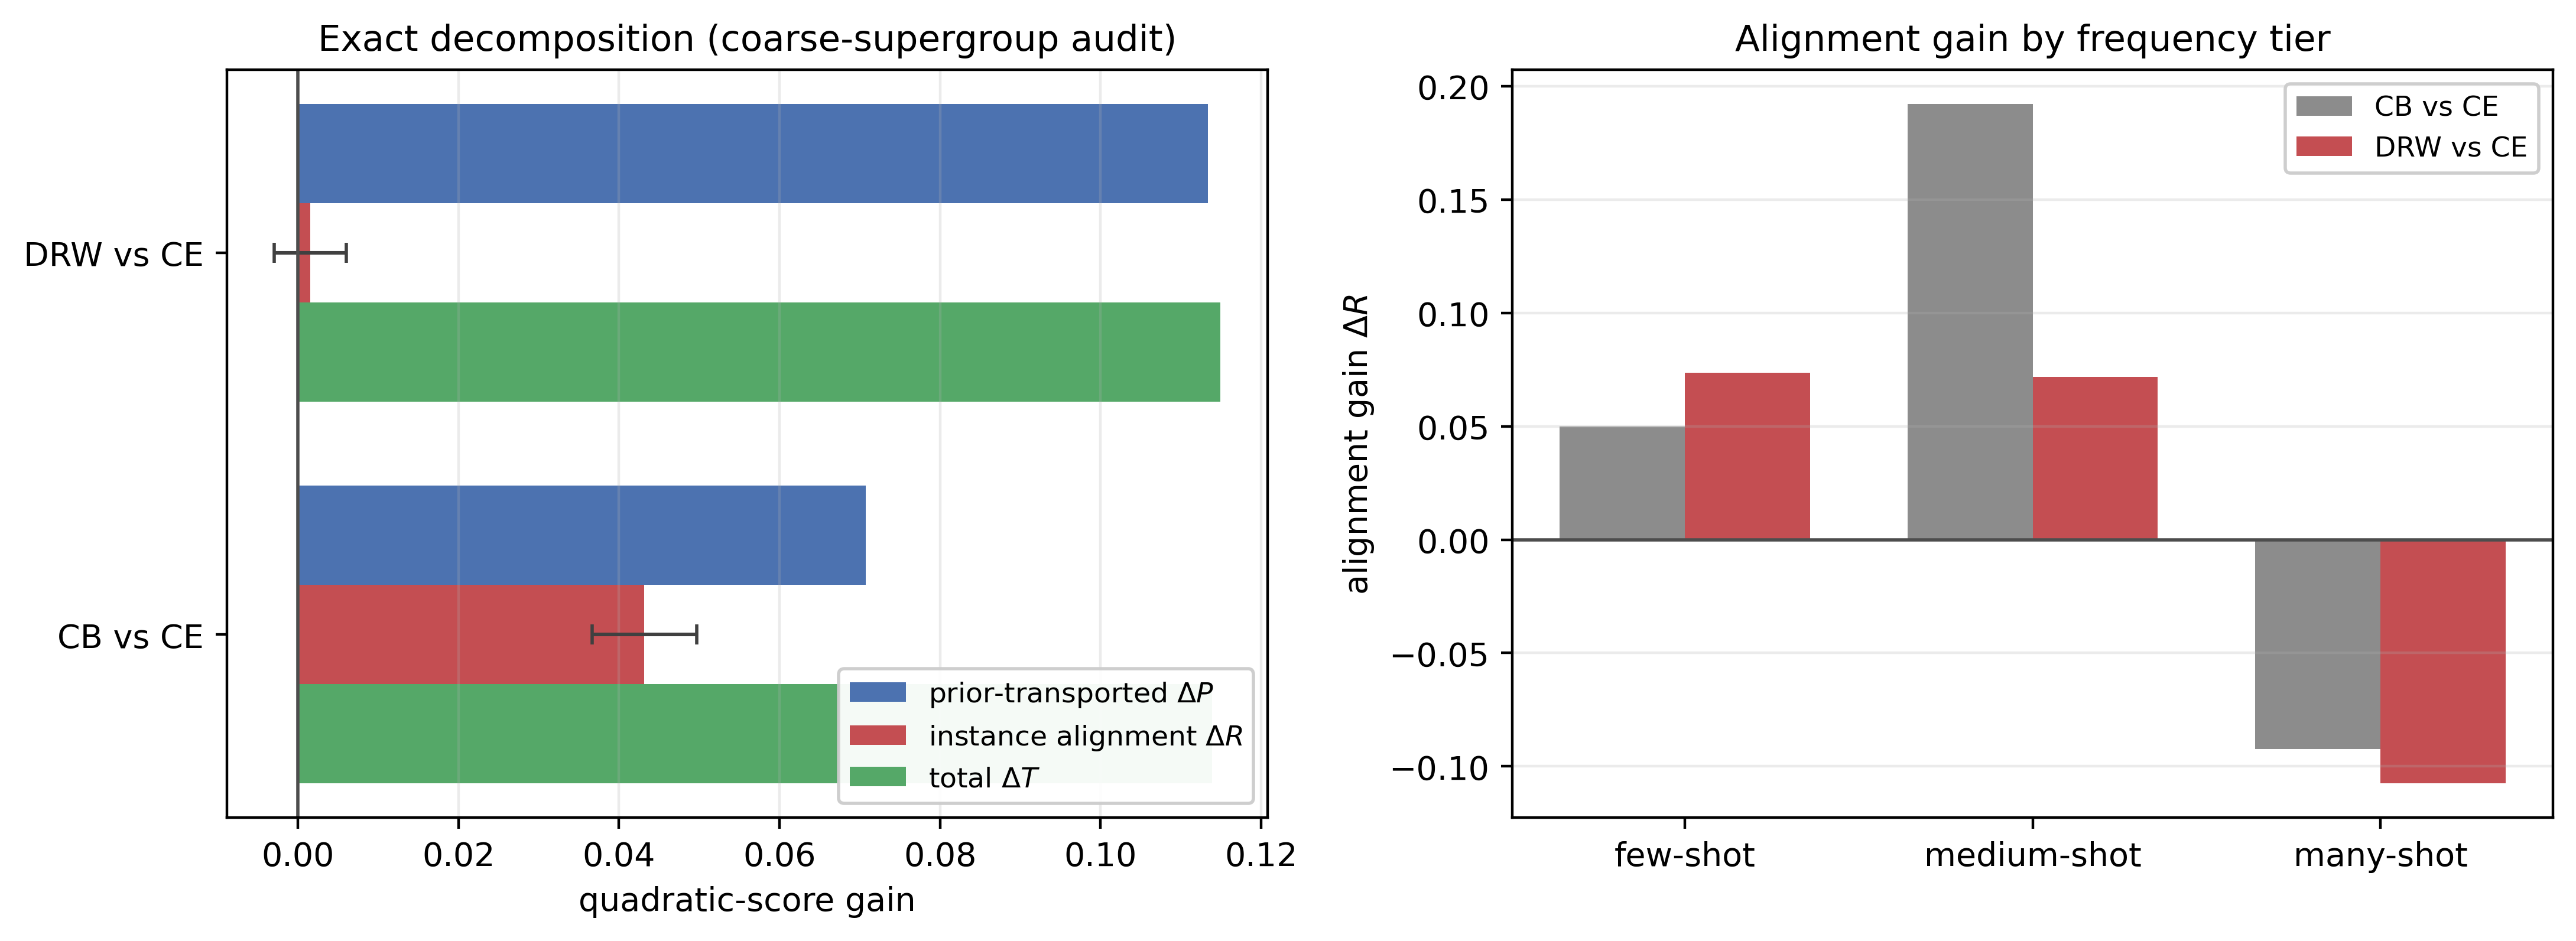
\includegraphics[width=\textwidth]{figures/fig8_text_lt.png}
\caption{\textbf{A third domain, with neither a spatial nor a class-frequency prior.}
Left: exact decomposition at the coarse-topic audit; CB's total gain is genuinely split
between both channels while DRW's is almost entirely prior-fit. Error bars are
95\% H\'ajek intervals on $\widehat{\Delta R}$. Right: resolution gain by
training-frequency tier for both schedules, showing the same head-loses/tail-gains
signature as Figure~\ref{fig:cifar} despite the change of domain and grouping variable.}
\label{fig:textlt}
\end{figure*}

Table~\ref{tab:textlt-tier} breaks the superclass-audit resolution down by
training-frequency tier for both schedules; the two methods agree in shape even though
their superclass totals diverge sharply in composition, each gaining resolution on rare
and medium-frequency categories and losing it on frequent ones, the same qualitative
signature Appendix~\ref{app:lt} reports for image classification.

\begin{table}[t]
\centering
\caption{Resolution gain by training-frequency tier at the superclass audit,
20-Newsgroups-LT. Both schedules gain within-group resolution on rare and medium categories
and lose it on frequent ones.}
\label{tab:textlt-tier}
\begin{tabular}{@{}lrrr@{}}
\toprule
Tier & $n$ & $\widehat{\Delta R}$, CB vs CE & $\widehat{\Delta R}$, DRW vs CE \\
\midrule
Few-shot ($<20$)          & 1954 & $0.04991$  & $0.07352$  \\
Medium-shot ($20$--$100$) & 2610 & $0.19213$  & $0.07171$  \\
Many-shot ($>100$)        & 2968 & $-0.09227$ & $-0.10753$ \\
\bottomrule
\end{tabular}
\end{table}

This third domain uses a single trained pair per schedule rather than the multi-seed,
calibration-matched protocol Appendix~\ref{app:lt} applies to CIFAR-100-LT; extending
that fuller protocol to text is the natural next replication, not a step this section
claims to have taken.
